\documentclass[iop]{emulateapj}
\usepackage{color}
\usepackage{natbib}
\usepackage{amsmath}
\bibliographystyle{apj}

\newcommand{\vdag}{(v)^\dagger}
\newcommand{\myemail}{eogorma@tcd.ie}

\shorttitle{Radio Emission Studies of Dust-free Red Giants}
\shortauthors{O'Gorman et al.}

\begin{document}

\title{Multi-wavelength Radio Continuum Emission Studies of Dust-free Red Giants}


\author{Eamon O'Gorman\altaffilmark{1}, Graham M. Harper\altaffilmark{1}, Alexander Brown\altaffilmark{2}, Stephen Drake\altaffilmark{3}, and Anita M. S. Richards\altaffilmark{4}}
\altaffiltext{1}{School of Physics, Trinity College Dublin, Dublin 2, Ireland}
\altaffiltext{2}{Center for Astrophysics and Space Astronomy, University of Colorado, 389 UCB, Boulder, CO 80309, USA}
\altaffiltext{3}{NASA Goddard Space Flight Center, Greenbelt, MD 20771, USA}
\altaffiltext{4}{Jodrell Bank Centre for Astrophysics, School of Physics and Astronomy, University of Manchester, Manchester M13 9PL, UK}

%\email{eogorma@tcd.ie}
%\email{graham.harper@tcd.ie}
%\email{alexander.brown@colorado.edu}
%\email{a.m.s.richards@manchester.ac.uk}
%\email{drake@milkyway.gsfc.nasa.gov}

\begin{abstract}

Multi-wavelength centimeter continuum observations of non-dusty, non-pulsating K spectral-type red giants directly sample their wind acceleration zones where most of the energy that drives their mass loss is deposited. Such stars are feeble emitters at these wavelengths however, and previous observations have provided only a small number of modest signal-to-noise measurements slowly accumulated over three decades. We present multi-wavelength Karl G. Jansky Very Large Array (VLA) thermal continuum observations of the wind acceleration zones of two dust-free red giants, Arcturus ($\alpha$ Boo: K2 III) and Aldebaran ($\alpha$ Tau: K5 III). Importantly, most of our observations were carried out within a few days of each other so any long term variability that may exist does not affect our analysis. We report the first detections at many wavelengths for each star including a detection at 10 cm (3.0 GHz: S-band) for both stars and a 20 cm (1.5 GHz: L-band) detection for $\alpha$ Boo. This is the first time single (non-binary) luminosity class III red giants have been detected at these wavelengths. These long wavelength flux density measurements sample the outer layers of the stars atmosphere where the wind velocity is approaching (or possibly has reached) its terminal value and the ionization balance is becoming \textit{frozen-in}. As a result, they are important empirical constraints for atmospheric models. We present spectral energy distributions for both stars and compare these with previous measurements and published semi-empirical models based on ultraviolet data. The marked deviations between our data and existing semi-empirical models highlight the need for new atmospheric models to be developed. Spectral indices are used to discuss the possible properties of the stellar atmospheres and we find evidence for a rapidly cooling wind in the case of $\alpha$ Boo. We develop a simple analytical atmospheric model for $\alpha$ Boo which includes a rapidly cooling constant velocity wind and is found to be in good agreement with our new long wavelength flux density values.

\end{abstract}

\keywords{Radio continuum: stars --- Stars: chromospheres --- Stars: individual ($\rm{\alpha}$ Boo, $\rm{\alpha}$ Tau) --- Stars: late-type --- Stars: winds, outflows}

\section{INTRODUCTION}

Mass loss from late-type evolved stars plays a crucial role in both stellar and galactic evolution and ultimately provides part of of the material required for the next generation of stars and planets. Despite the importance of this phenomenon and decades of study, the mechanisms that drive winds from evolved spectral-type K through mid-M stars remain an enduring mystery [clearly laid out by \cite{1985ASSL..117..229H} but still unsolved, e.g., \cite{2009AIPC.1094..267C}]. There is insufficient atomic, molecular, or dust opacity to drive a radiation-driven outflow and acoustic/pulsation models cannot drive the observed mass loss rates \citep{1995ApJ...442L..61S}. Optical and ultraviolet observations reveal an absence of hot wind plasma and the winds are thus too cool to be Parker-type thermally-driven flows \cite[e.g.,][]{1979ApJ...229L..27L,1981ApJ...250..293A}. 

Magnetic fields are most likely involved in the mass loss process, although current magnetic models are also unable to explain spectral diagnostics. Exquisite high signal-to-noise (S/N) ratio \textit{Hubble} ultraviolet (UV) spectra have revealed that the 1-D linear Alfv\'en wave-driven wind models of the 1980’s (e.g., \citealt{1980ApJ...242..260H,1988PhDT........13H}) are untenable. These models predict chromospheres as integral parts of a turbulent, extended and heated wind acceleration zone, but the theoretical line profiles and electron densities do not agree with the \textit{Hubble} spectra, \cite[e.g.,][]{1998ApJ...494..828J}. One important property of cool evolved star winds gleaned from UV spectra is that, for the most part, the red giant winds accelerate in a quasi-steady manner and are not the result of ballistic ejecta as shown by the increase of wind scattering absorption with optical depth in Fe II lines \citep{1999ApJ...521..382C}. A new generation of theoretical models with outflows driven within diverging magnetic flux tubes have now emerged \citep{2006MNRAS.368.1145F, 2007ApJ...659.1592S} but these too are not yet in agreement with observations \citep{2009AIPC.1094..267C}. It has also been suggested that the winds may be driven by some form of magnetic pressure acting on very highly clumped wind material \citep{2008AJ....136.1964E} but \cite{2010ApJ...720.1767H} does not find support for this hypothesis. Progress in this field continues to be driven by observations that provide new insights into the mass loss problem.

\subsection{Radio Continuum Observations} \label{intro1} 

Although studies of wind-scattered UV and optical line profiles have provided clues to the mass loss rates and radial distribution of the mean and turbulent velocity fields, the thermal structure remains poorly constrained. In the UV, the source function of electron collisionally excited emission lines is sensitive to electron temperature (i.e., $S_{\nu} \propto e^{-h\nu /kT}$) and so a localized hot plasma component in a dynamic atmosphere can completely dominate the temporally and spatially averaged emission and not hence reflect the global mean value. At radio wavelengths however, the source function is thermal and is just the Rayleigh-Jeans tail of the Planck function, which is linear in electron temperature (i.e., $S_{\nu} = {2kT\nu ^2 /c^2}$) and so should give a more appropriate estimate of the mean thermal wind structure. It is this value that controls the atomic level populations and ionization of the mean plasma that feed into UV spectroscopic analyses. This value is also needed to quantify the implied thermal heating supplied to the  wind by the unknown driving source/sources, allowing constraints on potential mass loss mechanisms to be derived.

In the cm-radio regime the radio opacity strongly increases with wavelength (i.e., $ \kappa _{\lambda} \propto \lambda ^{2.1}$) and so the longer wavelengths sample the extended layers of a stars atmosphere, thus	 providing us with spatial information about the star's mass outflow region. The NRAO\footnote{The National Radio Astronomy Observatory is a facility of the National Science Foundation operated under cooperative agreement by Associated Universities, Inc.} Karl G. Jansky Very Large Array (VLA) offers over three orders of magnitude in continuum optical depth ($\tau _{20 \ \rm{cm}}/\tau _{0.7 \ \rm{cm}} \approx 10^3$) and provides an area-averaged sweep through the wind acceleration zones of evolved late type stars. The thermodynamic properties in this spatial region control the ionization in the far wind because the ionization balance, which also controls the cooling rates, becomes \textit{frozen-in} at large radii due to advection. Furthermore, it is these outer extended regions of the star's atmosphere that contribute to the commonly seen P Cygni line profiles in the UV. In these profiles the line-of-sight absorption caused by the star's wind is superimposed on the blueshifted scattered emission. Thus, centimeter radio continuum observations can provide a test of models based on these UV profiles. In this paper we directly compare our new VLA observations with atmospheric models derived from UV analysis.

\subsection{Sample Selection} \label{intro2}

Currently the most detailed spatial information about the atmospheres of K and early M evolved stars is obtained from eclipsing binaries such as the $\zeta$ Aurigae and symbiotic systems (e.g., \citealt{1970VA.....12..147W}; \citealt{1996ApJ...466..979B}; \citealt{2008AJ....136.1964E}; \citealt{2008ApJ...675..711C}). Even though these systems offer us the best opportunity to obtain information on the dynamics and thermodynamics at various heights in the evolved star's atmosphere, the very nature of the binary system may introduce further complexities. For example, the orbital separation is often within the wind acceleration region and one could expect flow perturbations to be present (e.g., \citealt{1981ApJ...248.1043C}). In fact, using the `old' VLA, \cite{2005AJ....129.1018H} confirm that the velocity structure of  of $\zeta$ Aurigae is not typical of single stars with similar spectral types, such as $\lambda$ Velorum \citep{1999ApJ...521..382C}. 

In order to avoid the assumed additional complexities of a companion, we have selected two single luminosity class III red giants: Arcturus ($\alpha$ Boo: K2 III) and Aldebaren ($\alpha$ Tau: K5 III). These nearby red giants have been extensively studied at other wavelengths and their stellar parameters, which are briefly summarized in Table 1, are accurately known. These stars are predicted to be point sources at all frequencies in all VLA configurations so our radio observations measure their total flux density, $F_{\nu}$. Moreover, both stars have existing semi-empirical 1-D chromospheric and wind models which we directly compare to our data in this paper. 

\begin{deluxetable}{ccc}
\tabletypesize{\scriptsize}
\tablecaption{Properties of red giant sample.}
\tablehead{	\colhead{}		       				& 
			\colhead{$\alpha$ Boo}				&
			\colhead{$\alpha$ Tau}				}
\startdata
Spectral Type 				& K2 III  & K5 III  \\
HD Number 				& 124897  & 29139  \\
Mass (M_{\odot})	& $0.8 \pm 0.2$  & $1.3 \pm 0.3$ \\
Effective Temperature (K)	& $4294 \pm 30$  & $3970 \pm 49$ \\
Angular Diameter (mas)		& $21.0 \pm 0.2$ & $20.2 \pm 0.3$ \\
Distance (pc)	& $11.3 \pm 0.1$ & $20.4 \pm 0.3$\\
Radius ($R_{\odot}$)	& $25.4 \pm 0.3$  & $44.4 \pm 1.0$ \\
Photospheric Escape Velocity & 110 km s$^{-1}$ & 106 km s$^{-1}$ \\
Wind Terminal Velocity & $\sim$40 km s$^{-1}$ & $\sim$30 km s$^{-1}$ \\
Mass Loss Rate ($M_{\odot}$ yr$^{-1}$)		& 2$\times$10$^{-10}$ & 1.6$\times$10$^{-11}$ \\
Wind Temperature (K)		& $\sim$10,000  & $< 10,000$  \\
Semi-empirical Model	& \cite{1985pssl.proc..351D} & \cite{1999MNRAS.302...37M}
\enddata
\tablecomments{Masses are from \cite{2010A&A...509A..77K} and \cite{2012A&A...547A.108L}. Effective temperatures and photospheric angular diameters are from \cite{1993AA...270..315D}. Distances are from \cite{2007A&A...474..653V}. Mass loss rates are from \cite{1985pssl.proc..351D} and \cite{1998ApJ...503..396R}.}

\label{tab:tab1}
\end{deluxetable}

\begin{deluxetable*}{ccccccccc}
\tabletypesize{\scriptsize}
%\tablecolumns{6} 
%\tablewidth{0pt} 
\tablecaption{VLA Observations}
\tablehead{\colhead{Star}			            &
\colhead{Date}
				&
          	\colhead{Band}	      				&
          	\colhead{Frequency\tablenotemark{a}}&
	\colhead{Wavelength}			         	&
           	\colhead{Time on Star}              &
           	\colhead{Bandwidth}            		&
           	\colhead{Number of}            		&
	\colhead{Phase}		\\
	\colhead{}									&
    \colhead{}		                			& 
    \colhead{}		                			& 
	\colhead{(GHz)}                        		& 
	\colhead{(cm)}                         		& 
	\colhead{(hr)}                    			&
	\colhead{(GHz)}                        		&
	\colhead{Antennae\tablenotemark{b}}         &
	\colhead{Calibrator}		}
\startdata
$\alpha$ Boo	& 2011 Feb 22 & Q	& 43.3 & 0.7		& 0.3 	&  0.256	&22& J1357+1919  \\
$\alpha$ Boo 	& 2011 Feb 22 & Ka	& 33.6 & 0.9		& 0.2 	&  0.256 	&23&J1357+1919  \\
$\alpha$ Boo 	& 2011 Feb 22 & K	& 22.5 & 1.3		& 0.4	&  0.256 	&24&J1357+1919  \\
$\alpha$ Boo 	& 2011 Feb 11 & X	& 8.5  & 3.5		& 0.3 	&  0.256 	&18&J1415+1320  \\
$\alpha$ Boo	& 2011 Feb 11 & C	& 5.0  & 6.0 		& 0.5	& 0.256 	&21& J1415+1320 \\
$\alpha$ Boo	& 2011 Feb 13 & S	& 3.1  & 9.5 		& 1.8 	& 0.256 	&12& J1415+1320 \\
$\alpha$ Boo 	& 2012 Jul 19 & S	& 3.0  & 10.0 		& 0.7 	& 2.0 		&23& J1415+1320 \\
$\alpha$ Boo	& 2012 Jul 20 & L	& 1.5  & 20.0		& 1.6 	& 1.0 		&23& J1415+1320 \\
$\alpha$ Tau	& 2011 Feb 11 & Q	& 43.3 & 0.7 		& 0.3 	& 0.256 	&22&  J0431+1731\\
$\alpha$ Tau	& 2011 Feb 11 & Ka	& 33.6 & 0.9 		& 0.2 	& 0.256 	&19&  J0449+1121\\
$\alpha$ Tau	& 2011 Feb 11 & K	& 22.5 & 1.3 		& 0.4 	& 0.256 	&21&  J0449+1121\\
$\alpha$ Tau	& 2011 Feb 13 & X	&  8.5 & 3.5 		& 0.5	& 0.256 	&25&  J0449+1121\\
$\alpha$ Tau	& 2011 Feb 13 & C	&  5.0 & 6.0 		& 1.2	& 0.256 	&21&  J0449+1121\\
$\alpha$ Tau	& 2011 Feb 12 & S	&  3.1 & 9.5 		& 1.8 	& 0.256 	&11&  J0431+2037
\enddata
\tablenotetext{a}{Central frequency of selected bandpass.}
\tablenotetext{b}{Number of available antennae remaining after flagging.}
\label{tab:tab2}
\end{deluxetable*}

\section{OBSERVATIONS AND DATA REDUCTION}

Observations of $\alpha$ Boo and $\alpha$ Tau were carried out with the VLA during Open Shared Risk Observing (OSRO) in February 2011 at Q, Ka, K, X, C, and S-band in B-configuration (PI: Harper; program 10C-105). $\alpha$ Boo was also observed at S and L-band in July 2012 when the VLA was again in B-configuration (PI: O'Gorman; program 12A-472). Some details of these observations are given in Table \ref{tab:tab2}. For the 2011 observations, the correlator was set up with two 128 MHz sub-bands centered on the frequencies listed in Table \ref{tab:tab2}. Each sub-band had sixty-four channels of width 2 MHz and four polarization products (RR, LL, RL, LR). For the S and L-band observations in 2012, the 1-2 GHz and 2-4 GHz frequency ranges were both divided into 16 sub-bands, each with sixty-four channels. The channel width was 2 and 1 MHz for S and L-band, respectively.

Both $\alpha$ Boo and $\alpha$ Tau were slightly offset from the phase-center by $\sim$5 synthesized beam widths in order to avoid possible errors at phase-center. All scheduling blocks (SBs) were kept to $\le$\,2.5 hours of duration. For the high frequency observations (i.e., Q, Ka, and K-bands) we used the \textit{fast switching} technique which consists of rapidly alternating observations of the target source and a nearby unresolved phase calibrator. The total cycle times for the Q, Ka, and K-band observations were 160, 230, and 290 s, respectively. For both target sources these high frequency observations were combined into a single 2 hour observing track and commenced with X-band reference pointing with solutions being applied on-line. After X-band pointing the target source was observed at Q-band to insure the best pointing solutions were used. The lower frequencies tracks were composed of repeatedly interleaving observations of the target source and a nearby phase calibrator but had longer cycle times. The primary calibration sources 3C286 and 3C138 were observed at the end of all tracks and were used to measure the complex bandpass and set the absolute flux for $\alpha$ Boo and $\alpha$ Tau, respectively.  

The data were flagged, calibrated, and imaged within the Common Astronomical Software Application  \cite[CASA;][]{2007ASPC..376..127M} package. Data deemed to be bad by the VLA online system were flagged, as were zeros, non-operational antennae, dummy scans at the beginning of each track, and poorly performing antennae. Visual inspection of each scan was carried out to determine if data at the beginning or end of these scans needed to be flagged. For the 2011 low frequency data the two sub-bands were centered at relatively radio frequency interference (RFI) free regions of the bandpass and only a very small amount of RFI had to be flagged.   The 2012 wide-band data were initially Hanning smoothed (combining adjacent frequency channels with weights 0.25, 0.5, and 0.25) to suppress Gibbs ringing. We manually flagged entire sub-bands that were badly contaminated with RFI. The \textit{testautoflag} task was then used to conservatively flag RFI from all sources and any remaining RFI was manually flagged. 

In order to calibrate the data, we solved for the complex gains of the calibration sources while applying the bandpass solution, which was derived from the relevant flux calibrator.  The amplitude gains of the phase calibrators were scaled according to values derived from the flux calibrators using the ``Perley-Butler 2010" flux density standard \citep{2013ApJS..204...19P}. At the time, no Ka or S-band flux density standard models were available so instead for these we used the K and L-band models, respectively. The more frequently observed phase calibrators were then used to calibrate the amplitude and phases of the targets. Atmospheric opacity corrections were also applied to the high frequency data sets using the average of a seasonal model (based on many years of measurements) and information from the weather station obtained during the observations.

The visibilities were then both Fourier transformed and deconvolved using the CASA \textit{clean} task in multi-frequency synthesis imaging mode, which separately grids the multiple spectral channels onto the \textit{u-v} plane and therefore improves the overall \textit{u-v} coverage. We used natural weighting for maximum sensitivity and the cell size was chosen so that the synthesized beam was about five pixels across. For the high frequencies it was usually sufficient to place just one CLEAN circle around the target source.  For the low frequencies however, the image sizes were usually set to a few times the size of the primary beam so that nearby strong serendipitous sources could be CLEANed thus reducing their sidelobe contamination of the final image. These images were CLEANed interactively, with w-term correction, down to about the $3\sigma$  level with clean boxes placed around sources as they appeared in the residual image. All images were corrected for  primary beam attenuation. 

In each image the flux density from the unresolved target source was calculated by, 1) taking the peak pixel value from the source, 2) manually integrating the flux density around the source, and 3) fitting an elliptical Gaussian model to the source and deriving the integrated flux density using the CASA \textit{imfit} task. Each of these values along with the image root mean square (rms) noise measured from adjacent background regions and fitting error produced by \textit{imfit} are given in Table \ref{tab:tab3}. For weak detections (i.e., $F_{\nu} \lesssim 5\sigma$) we avoid using the \textit{imfit} task to obtain a flux density estimate, as this may produce biased parameter estimates \citep{1999ASPC..180.....T}. The flux density values used in Section \ref{disc:disc0} are the peak values listed in Table \ref{tab:tab3}. We assume absolute flux density scale systematic uncertainties of  3\% at all frequencies \citep{2013ApJS..204...19P}.

\begin{deluxetable*}{Cccccccc}
\tabletypesize{\scriptsize}
%\tablecolumns{6} 
%\tablewidth{0pt} 
\tablecaption{VLA Fluxe Densities of $\alpha$ Boo and $\alpha$ Tau}
\tablehead{\colhead{}		            &
			\colhead{Band}		            &
			\colhead{Frequency\tablenotemark{a}}&
			\colhead{Peak $F_{\nu}$}					&
          	\colhead{Integrated $F_{\nu}$} 			&
          	\colhead{\textit{Imfit} Integrated}	&
			\colhead{Image rms}					&
           	\colhead{\textit{Imfit} Fitting}  	\\
	\colhead{}									&
	\colhead{}									&
	\colhead{(GHz)}								&
    \colhead{(mJy)}		        	& 
    \colhead{(mJy)}		                		& 
	\colhead{$F_{\nu}$ (\rm{mJy})}                        		& 
	\colhead{(Jy beam^{-1})}         					&
	\colhead{Error (mJy)}		}
\startdata
$\alpha$ Boo (K2 III) &Q  &43.28& 5.941 & 6.093 & 6.420 & 0.301 &  0.261\\
&Ka &33.56& 4.159 & 4.319 & 4.489 & 0.083 & 0.090 \\
&K  &22.46& 1.827 & 1.784 & 1.809 & 0.043 & 0.050 \\
&X  &8.46 & 0.510 & 0.514 & 0.532 & 0.030 & 0.019 \\
&C  &4.90 & 0.214 & 0.144 & 0.159 & 0.035 & 0.009 \\
&S  &3.15 & 0.148 & 0.135 & -     & 0.028 & -     \\
&S  &2.87 & 0.127 & 0.118 & 0.116 & 0.012 & 0.016\\
&L  &1.63 & 0.067 & 0.068 & -     & 0.013 & -    \\
\hline
\rule{0pt}{3ex}  $\alpha$ Tau (K5 III)&Q  &43.28 & 3.672& 3.734 & 4.082 &  0.259& 0.183	\\
&Ka &33.56 & 2.188& 1.962 & 2.125 &  0.091& 0.070 \\
&K  &22.46 & 1.864& 1.881 & 2.069 &  0.042& 0.083 \\
&X  &8.46  & 0.296& 0.287 & 0.281 &  0.014& 0.015 \\
&C  &4.96  & 0.147& 0.167 & 0.176 &  0.010& 0.010 \\
&S  &3.15  & 0.062& 0.043 & - &  0.017 & -
\enddata
\tablenotetext{a}{Frequency of the final image produced using the multi-frequency synthesis imaging mode within CASA's \textit{clean} task.}
\label{tab:tab3}
\end{deluxetable*}

\section{RESULTS} 

Apart from $\alpha$ Boo at C-band and $\alpha$ Tau at S-band, detections were made in both sub-bands for the 2011 data. For all other bands, the flux densities of the targets in both sub-bands were found to be the same within their uncertainties so we do not present these values here. Instead we give the values from the radio maps produced by concatenating the two sub-bands. We present in Table \ref{tab:tab3} the target flux densities extracted from these concatenated radio maps. In the following two sections we briefly discuss the properties of these radio maps for both targets.

\subsection{$\alpha$ Boo Radio Maps} \label{results1} 
High S/N detections ($>19\sigma$) of $\alpha$ Boo were made at 22.5, 33.6, and 43.3 GHz. Some residuals of the dirty beam remained in the CLEANed maps due to the paucity of uv-coverage in these short high frequency observations. The lower frequencies maps were contaminated by the emission of a strong radio source located $186\arcsec$ north-west of $\alpha$ Boo. This source was reported by \cite{1986AJ.....91..602D} and their flux density of 25 mJy at 4.9 GHz is in close agreement with our measurement of 23.2 mJy at the same frequency. We find the source to have a spectral index $\alpha$ ($F_{\nu} \propto \nu ^{\alpha}$), equal to -1.4 and reaches 80.3 mJy at 1.6 GHz. For unknown reasons we do not detect $\alpha$ Boo in the higher frequency sub-band at 5.0 GHz (C-band) so the values given in Table \ref{tab:tab3} are taken from the lower frequency sub-band only. We obtain good detections ($>5\sigma$) of the star for both epochs at $\sim$3 GHz (S-band) and the peak flux densities agree within their uncertainties. We can therefore safely assume that the 1.5 GHz (L-band) flux density has not changed significantly over that period either, and so can safely be included in any analysis. The map at L-band was highly contaminated by the sidelobes of the strong source north-west of $\alpha$ Boo but the star is still detected at the $5\sigma$ level. There is a slight positional offset of $1\arcsec$ between the position of the peak flux density at 1.5 and at 3.0 GHz for the 2012 data, which were taken within 1 day of each other. However, this is less than a quarter of the 1.5 GHz synthesized beam and considering that the $4\sigma$ contours overlap, we feel that it is highly unlikely that both sources are not $\alpha$ Boo. 

\subsection{$\alpha$ Tau Radio Maps} \label{results2}
The final deconvolved radio maps of $\alpha$ Tau were of excellent quality with the rms noise reaching the predicted noise levels in many cases. The target field at all frequencies was free from strong serendipitous radio sources and thus the final images were free of the sidelobe contamination that were present in the low frequency $\alpha$ Boo images. $\alpha$ Tau was the only source in the high frequency maps while the brightest source in the low frequency maps was located $106\arcsec$ north north-east of $\alpha$ Tau and had flux densities of 0.85, 1.35, and 1.7 mJy at 8.5, 5.0, and 3.5 GHz, respectively. Strong detections ($>14\sigma$) of $\alpha$ Tau were made at all frequencies between 5.0 and 43.3 GHz. Due to the limited number of S-band receivers available at the time, a full 2.5 hr track was dedicated to $\alpha$ Tau at 3.1 GHz in order to achieve the required sensitivity to give a possible detection. We report a tentative $3\sigma$ detection of $\alpha$ Tau at 3.1 GHz when we take its peak pixel value as its total flux density. 

\begin{deluxetable*}{cccccc}
\tabletypesize{\scriptsize}
%\tablecolumns{6} 
%\tablewidth{0pt} 
\tablecaption{Compilation of Previous Radio Observations of $\alpha$ Boo and $\alpha$ Tau ($\nu \le 250$ GHz)}
\tablehead{							            &
    \colhead{$\nu$ (GHz)}		       				& 
			\colhead{Date}						&
			\colhead{$F_{\nu}$ (mJy)}				&
			\colhead{$F_{\nu}/\sigma$}				&
          	\colhead{Source} 					}
\startdata
$\alpha$ Boo (K2 III) &4.9  & 1983 Jan 21 & 0.39 & 3.0 & \cite{1986AJ.....91..602D} \\
&4.9  & 1983 May 20 & 0.26 & 3.3& \cite{1986AJ.....91..602D} \\
&4.9  & 1983 Dec 26 & $\le 0.18 \ (3\sigma)$&- & \cite{1986AJ.....91..602D} \\
&4.9  & 1984 Mar 17 & 0.24  & 4.8& \cite{1986AJ.....91..602D} \\
&15.0 & 1984 Nov 6 & 0.68 & 7.6& \cite{1986AJ.....91..602D} \\
&22.5  & 1999 Jan 06  &1.7& 8.5& \cite{2011AA...533A.107D} \\
&43.3  & 1999 Jan 06 & 3.3& 8.3& \cite{2011AA...533A.107D} \\
&43.3  & 2004 Jan 25 & 3.34& 41.8& \cite{2011AA...533A.107D} \\
&86.0  & 1985 Nov  & 21.4& 3.0& \cite{1986AA...164..227A} \\
&108.4  & 1997 Nov - 2000 Jun & 20.1 &29.1 & \cite{2005AJ....129.2836C} \\
&217.8 & 1997 Nov - 2000 Jun  & 83.5 &48.8 & \cite{2005AJ....129.2836C} \\
&250.0  & 1986 Dec - 1989 Mar  & 78.0 & 9.8& \cite{1994AA...281..161A} \\
\hline
\rule{0pt}{3ex}    $\alpha$ Tau (K5 III)	&4.9  & 1983 Jan 21 & $\le 0.27 \ (3\sigma)$&-& \cite{1986AJ.....91..602D} \\
&4.9  & 1984 Nov 6 & $\le 0.22 \ (3\sigma)$&-& \cite{1986AJ.....91..602D} \\
&5.0  & 1997 Sep 27 & $\le 0.07 \ (3\sigma)$	&-& \cite{2007ApJ...655..946W} \\
&8.5  & 1997 Sep 27 & 0.28 	&9.3	& \cite{2007ApJ...655..946W} \\
&14.9 & 1997 Sep 27 & 0.95 	&11.9	& \cite{2007ApJ...655..946W} \\
&15.0 & 1984 Nov 6 & 0.60 	&6.0	& \cite{1986AJ.....91..602D} \\
&108.4  & 1997 Nov - 2000 Dec &  14.0  & 9.6& \cite{2005AJ....129.2836C} \\
&217.8 & 1999 Sep - 2000 Dec  & 25.8 & 4.6& \cite{2005AJ....129.2836C} \\
&250.0  & 1986 Dec - 1987 Jan & 51.0 & 8.5& \cite{1994AA...281..161A} 
\enddata
\label{tab:tab4}
\end{deluxetable*}

\section{DISCUSSION} \label{disc:disc0}
\subsection{Results Versus Previous Observations} \label{disc1}
Prior to and during the early operation of the `old' VLA, a small number of single dish radio observations reported the detection of flares from single red giants (e.g., \citealt{1981ApJ...245L..71B}). These transient radio events have never been re-observed however, even with more sensitive interferometers, suggesting that such detections were false (e.g., \citealt{1992MNRAS.254....1B}). The first definitive detection of thermal free-free emission from a luminosity class III single red giant at centimeter wavelengths was of $\alpha$ Boo at 6 cm \citep{1983ApJ...274L..77D,1986AJ.....91..602D}. Since then there has been a modest number of centimeter and millimeter observations of this star. In Table \ref{tab:tab4} we list the majority of these observations and plot their flux densities as a function of frequency in Figure \ref{fig:fig1}. In comparison to other single red giants, $\alpha$ Boo had been relatively well observed at radio continuum wavelengths before this study, including detections in four VLA bands (i.e., Q, K, Ku, and C). No Ku band receivers were available during the commissioning phase of the VLA in early 2011 so we can compare three of our detections with previous ones. 

Previous detections of $\alpha$ Boo at 6 cm ranged from a 3$\sigma$ upper limit of 0.18 mJy to a 3$\sigma$ detection at 0.39 mJy. Our 6 cm value agrees to within $\sim$10$\%$ of the highest S/N (5$\sigma$) value of \cite{1986AJ.....91..602D}. There is no significant difference between our 1.3 cm value and that of \cite{2011AA...533A.107D}. There is however a notable difference in flux density values at 0.7 cm  where \cite{2011AA...533A.107D} report values that are lower than ours by over 40\%. Such a level of chromospheric variability seems rather high and would be unexpected from such supposedly inactive stars \citep{2013MNRAS.428.2064H}. Another possibility for the difference in values is that the longer cycle time used by \cite{2011AA...533A.107D}, which was over double our value, may cause larger phase errors and thus lower final flux density values. Future high frequency VLA observations of $\alpha$ Boo will clarify this discrepancy at 0.7 cm but past detections at longer wavelengths appear to be in good agreement with our data.

Prior to this study, $\alpha$ Tau had only been detected at two VLA bands (i.e., X and Ku) and had never been detected at wavelengths longer than 3 cm due to its weakly ionized wind and low mass-loss rate. Our lack of a Ku-band measurement means that we can only compare the previous 3 cm detection reported in \cite{2007ApJ...655..946W} to ours. We find that there is no significant difference between the two. Interestingly, \cite{2007ApJ...655..946W} report a non-detection of $\alpha$ Tau at 6 cm and placed a 3$\sigma$ upper limit of 0.07 mJy on its emission. In stark contrast to this, we were able to detect the star at 6 cm with a flux density over two times greater than this value. This hint of variability at long wavelengths can only again be confirmed with future high S/N observations.


\subsection{Existing Atmospheric Models} \label{disc2}
One of the most important diagnostic features indicating mass outflows in late type stars are the blue shifted absorption components present in the Mg {\textsc{ii}} h and k resonance lines. Figure \ref{fig:fig1} shows the predicted radio spectrum from the chromosphere and wind models of \cite{1985pssl.proc..351D}, which were based on the Mg {\textsc{ii}} k 2796 $\rm{\AA}$ emission line taken with the International Ultraviolet Explorer. We compute the radio spectrum from these models, assuming spherical 1-D geometry and the Gaunt factors from \cite{1988ApJ...327..477H} with free-free and H- free-free capacities included. The radiative transfer equation is solved using the Feautrier technique \cite[see, e.g.,][]{1994MNRAS.268..894H} and the boundary condition is determined by ensuring the atmosphere is optically thick at the deepest layers. Our computed radio spectrum reproduces Drake's (1985) predicted flux density value of $\sim$0.4 mJy at 6 cm and this is a good check on the robustness of our method of producing radio spectra from these model atmospheres. 

Both of Drake's atmospheric models contain the photospheric model of \cite{1975ApJ...200..660A} and predict the wind to reach a terminal velocity $v_{\infty}$, of $\sim$40 km s${}^{-1}$ by 2 $R _{\star}$. They contain a broad temperature plateau with T $\approx$ 8,000 K between 1.2 and $\sim$20 $R _{\star}$ with a cooler region further out. At high frequencies the radio spectra produced by these models have a blackbody-like slope (i.e., $\sim\nu ^{2}$) as a result of the small ion density scale heights close to the star where the temperature is changing slowly. At low frequencies however, where the models predict the wind to have constant velocity, ionization fraction and temperature, the slopes approaches the well known $\sim\nu ^{0.6}$ limit \citep{1975MNRAS.170...41W,1975AA....39..217O,1975AA....39....1P}. The paucity and, in some cases low S/N, of previous observations made it difficult to discern the validity of this model prior to our multi-frequency study of $\alpha$ Boo. Our new data reveal significant deviations from the semi-empirical model at both low and high frequencies (in this case below $\sim$8 GHz and above $\sim$25 GHz). At high frequencies our VLA data indicates a flux excess which is in agreement with previous mm-observations. The  discrepancy at low frequencies may indicate that we are still sampling a region of the wind where it is still accelerating (i.e., it has not yet reached its terminal velocity) or may also be a manifestation of rapid wind cooling further out than that predicted in UV spectral analysis. We will discuss these possibilities in the following sections.

\begin{figure*}
\centering
\includegraphics[trim = 0mm 0mm 0mm 20mm, clip,scale=0.65, angle=90]{fig1.ps}
\\
\caption{Spectral energy distribution of $\alpha$ Boo for 1 GHz $\leq \nu \leq$ 1 THz. Our new multi-frequency VLA observations which were mainly acquired over a few days in February 2011 are the blue circles and are in disagreement with the existing chromospheric and wind models of \cite{1985pssl.proc..351D}. The overlap between the two models are represented by the green shaded area. The red triangles are previous observations which were acquired sporadically over the last three decades with the `old' VLA, IRAM and BIMA. The black dashed line is the expected radio emission from the Drake model which undergoes rapid wind cooling beyond $\sim$2.3 $R_{\star}$ (see Section \ref{disc:disc3} and \ref{disc:disc4}).}
\label{fig:fig1}
\centering
\includegraphics[trim = 0mm 0mm 0mm 20mm, clip,scale=0.65, angle=90]{fig2.ps}
\\
\caption{Spectral energy distribution of $\alpha$ Tau for 1 GHz $\leq \nu \leq$ 1 THz. Our new multi-frequency VLA observations of $\alpha$ Tau (blue circles) were acquired in just two days in February 2011. The red triangles are the previous radio observations of the star which were acquired over many years. The green line is the expected radio emission from the existing hybrid chromosphere and wind model while the dashed  green line is the expected radio emission from a theoretical Alfv\'en wave driven model atmosphere.}
\label{fig:fig2}
\end{figure*}

In Figure \ref{fig:fig2} we plot the expected radio spectrum of $\alpha$ Tau based on the semi-empirical 1-D chromospheric model of \cite{1999MNRAS.302...37M} embedded in the 1-D wind model of \cite{1998ApJ...503..396R}. The McMurry model, which contains  the photospheric model of \cite{1973ApJ...180...81J}, is based on high S/N Hubble UV spectra and reaches a maximum temperature of 10$^{5}$ K at 1.2 $R_{\star}$. Beyond 1.2 $R_{\star}$ we use Robinson's wind characteristics to describe the outflow velocity where the wind reaches $\sim$80\% of its terminal value by 3 $R_{\star}$. We assume the wind to have a constant temperature of 8,000 K and have a constant ionization fraction, $x_{e}$, of 0.01 throughout. The combination of both atmospheric models result in a predicted excess of radio flux density at high frequencies (i.e., $\nu >$ 30 GHz) but does well in reproducing the VLA flux densities below 30 GHz. The VLA, Institut de Radioastronomie Millim\'{e}trique (IRAM) 30 m-telescope and Berkeley Illinois Maryland Association (BIMA) continuum flux densities confirm that this model predicts a flux excess at even higher frequencies. One possible explanation for this is that the inner atmosphere contains extensive cooler gas than that predicted by the 1-D static chromospheric model of McMurry. This scenario agrees with the findings of \cite{1994ApJ...423..806W} who conclude that cool regions exist close to the stellar surface with large filling factors i.e., a thermally bifurcated CO-mosphere.

We also include the predicted radio spectrum from the theoretical Alfv\'{e}n wave-driven outflow model for $\alpha$ Tau \citep{1989AcA....39..51K} in Figure \ref{fig:fig2} to demonstrate how radio observations can test the robustness of theoretical models. This model is based on a larger than now expected mass loss rate for the star (i.e., 6.3$\times$10$^{-9}$ M{$_{\odot$}} yr$^{-1}$) and predicts a fully ionized outflow with $v_{\infty} \approx 115$ km s$^{-1}$. As the radio opacity is proportional to $n _{\rm{e}} n _{\rm{ion}}$ this model greatly overestimates the actual radio flux density at all VLA wavelengths. The same result is to be expected from the Alfv\'{e}n wave models of $\alpha$ Boo \citep{1988AcA....38..107K} which are also fully ionized and have larger mass loss rates and outflow velocities than the established values given in Table \ref{tab:tab1}.

\subsection{Radio Spectral Indices} \label{disc:disc3}
The radio emission from non-dusty K spectral-type red giants is due to thermal free-free emission in their partially ionized outflows. The radio flux density-frequency relationship for these type of stars is always found to be intermediate between that expected from the stellar disk emission, where $\alpha$ follows the Rayleigh-Jeans tail of the Planck function (i.e., $\alpha = +2$), and that from an optically thin plasma ($\alpha = -0.1$). It can be shown that the expected radio spectrum from a spherically symmetric isothermal outflow with a constant velocity and ionization fraction varies as $\nu ^{0.6}$ \citep{1975MNRAS.170...41W,1975AA....39..217O,1975AA....39....1P}. If we relax some of the assumptions about the outflow in this constant property wind model and instead assume that the electron density and temperature vary as a function of distance from the star $r$, and have the power-law form $n_{e} \propto r^{-p}$ and $T_{e} \propto r^{-n}$ respectively, then 

\begin{figure}
\includegraphics[trim = 0mm 0mm 0mm 10mm, clip,scale=0.385,angle=90]{fig3.ps}
\caption{Radio spectra for $\alpha$ Boo and $\alpha$ Tau, together with the best fit straight lines to their long wavelength flux densities and the resulting spectral indices.}
\label{fig:fig3}
\end{figure}

\begin{equation}
\alpha = \frac{4p -6.2 -0.6n}{2p-1-1.35n}
\label{eq:eq1}
\end{equation}
\citep[e.g.,][]{1987ApJ...312..813S}. 

The radio spectra for both stars are shown in Figure \ref{fig:fig3}, together with the straight lines that were fitted to the long wavelength flux densities by minimizing the chi-square error statistic. For $\alpha$ Boo a power law with $F_{\nu} \propto \nu ^{1.05 \pm 0.05}$ fits the four longest wavelength data points well. This spectral index is larger than the 0.8 value obtained by \cite{1986AJ.....91..602D} whose value was based on a shorter wavelength (2 cm) value and a mean value of four low S/N measurements at 6 cm. $\alpha$ Tau was found to have a larger spectral index and a power law with $S_{\nu} \propto \nu ^{1.58 \pm 0.25}$ best fitted the three longest wavelength data points. This value is in agreement with \cite{1986AJ.....91..602D} who report a value $\ge 0.84$ and is lower than the value of 2.18 that can be derived from the shorter wavelength data given in \cite{2007ApJ...655..946W}. It should be emphasized that the spectral index for both stars is steeper than that expected from the constant property wind model. 

\begin{figure}
\includegraphics[trim = 0mm 11mm 0mm 21mm, clip,scale=0.4,angle=90]{fig4.ps}
\caption{The variation of density and temperature coefficients for the empirically derived spectral indices. The density coefficients for an isothermal flow along with the temperature coefficients for a constant outflow velocity are also shown for both stars.}
\label{fig:fig4}
\end{figure}

Equation \ref{eq:eq1} can be used in conjunction with our new spectral index for each star to calculate possible density and temperature coefficients that describe their outflow. The degree of variation of these coefficients with respect to one another are shown in Figure \ref{fig:fig4}. One explanation for spectral indices of stellar outflows being larger than 0.6 is that the wind is still accelerating in the region where the radio emission is emanating from and thermal gradients are assumed to be small. Ignoring thermal gradients may be reasonable over the small distances in which the red giants outflow undergoes rapid acceleration. If we too make this assumption then the density coefficients are $p=$2.71 and 5.5 for $\alpha$ Boo  and $\alpha$ Tau, respectively. This assumption is reasonable at short wavelengths where the majority of the radio emission is expected to emanate within the wind's acceleration zone, but at long VLA wavelengths (i.e., between 6 and 20 cm) we may indeed be sampling the wind very close to or at its terminal velocity and the wind may be have substantial thermal gradients. 

\begin{figure}
\includegraphics[trim = 5mm 0mm 10mm 20mm, clip,scale=0.4,angle=90]{fig5.ps}
\caption{Predicted effective radius (dashed lines) as a function of wavelength derived from the existing atmospheric models of $\alpha$ Boo and $\alpha$ Tau.  Also plotted is the predicted effective radius derived from our analytical advection model discussed in \ref{disc:disc4}. Points corresponding to our long wavelength VLA measurements are also shown. At the same radio wavelengths the less ionized and less opaque mass outflow of  Tau results in a smaller effective radius than $\alpha$ Boo.}
\label{fig:fig5}
\end{figure}

To investigate this matter further,  we estimate the effective radius of the radio emitting region per wavelength based on the Drake model for $\alpha$ Boo and the hybrid McMurry and Robinson model for $\alpha$ Tau. We follow the approach used by \cite{1977ApJ...212..488C} and assume that the radio emission at each wavelength emanates from a surface at radial optical depth $\tau _{\rm{rad}}=$1/3. This is just the Eddington-Barbier relation for an extended atmosphere where emission from smaller optical depths gets added weight. Since the radio free-free opacity increases at longer wavelengths (i.e., $\kappa _{\lambda} \propto \lambda ^{2.1}$) the optical depth along a line of sight into the stellar outflow also increases at longer wavelengths. This implies that the effective radius (i.e., the radius where $\tau _{\lambda} = \tau _{\rm{rad}}$) will increase with longer wavelengths and will be greater for outflows with higher ionization densities as $\tau _{\lambda} \propto \int \lambda ^{2.1}n_{\rm{ion}}n_{\rm{e}} dr$. 

The higher degree of ionization in the mass outflow of $\alpha$ Boo in comparison to $\alpha$ Tau makes a substantial difference to the size of the stars effective radius as can be seen in Figure \ref{fig:fig5}. At 6, 13, and 20 cm the effective radius of $\alpha$ Boo at $\tau _{\rm{rad}}$=1/3 is predicted to be 1.6, 2.8, and 3.7 $R_{\star}$ but is only $\sim$1.2 $R_{\star}$ at 6 and 13 cm for $\alpha$ Tau. \cite{1998ApJ...503..396R} predict that $\alpha$ Tau's wind reaches $\sim$80\% of its terminal velocity by 3 $R_{\star}$ so it is highly unlikely that even our longest wavelength VLA measurements of $\alpha$ Tau sample its outer wind. For $\alpha$ Boo however, \cite{1985pssl.proc..351D} predicts that the wind has reached its terminal velocity by $\sim$2 $R_{\star}$ so based on this model our longest VLA measurements probable sample the wind at, or very close to, its terminal velocity. Assuming this to be the case, Equation \ref{eq:eq1} then indicates that $\alpha$ Boo's steady outflow undergoes rapid cooling at a few stellar radii. The derived temperature coefficient of 1.65 points to a temperature power-law falloff exceeding that from a wind adiabatically cooling with no heat source (i.e. n=1.33 in this case) with the excess cooling being possible due to recombination of H$^{+}$ or heavier ions. Finally, if the wind ionization balance has not yet become \textit{frozen-in} in the region of $\alpha$ Boo's wind where the radio emission emanates from then the excess slope of the spectral index could be due to a combination of both cooling and changing ionization balance. In this scenario the temperature coefficient may be smaller then our derived value here.

\subsection{Analytical Advection Model for $\alpha$ Boo's Wind} \label{disc:disc4}

A failure of the existing atmospheric model for $\alpha$ Boo is that is overestimates the radio fluxes at long VLA wavelengths which sample its outer atmosphere, as clearly shown in Figure \ref{fig:fig1}. If these wavelengths are indeed sampling the wind at its terminal velocity then a reason for this overestimation may be that the wind is cooling closer in than that predicted by the existing models, which assumes a constant temperature of 8,000 K out to $\sim$20 $R_{\star}$. The main mechanism for this cooling would be adiabatic expansion \citep{2011ASPC..448..691O} and would cause lower electron densities than those predicted by the existing model due to larger recombination rates. To investigate this possibility further we adjusted one of the existing models [referred to `Model B' in \cite{1985pssl.proc..351D}] to include a temperature power-law falloff of the form
\begin{equation}
T_{e}(r)= T_{e}(r_{1})\left(\frac{r_{1}}{r}\right)^{1.65},
\label{eq:eq2}
\end{equation}
at some distance $r_{1}$, from the star. The temperature coefficient used here is that obtained from our new VLA data assuming a steady flow (see Figure \ref{fig:fig4}). To calculate the new $n_{\rm{e}}$ and $n_{\rm{ion}}$ densities in the wind regime where this temperature falloff occurs, we used the analytical expression of \cite{1986ApJ...306..605G} to calculate the hydrogen ionization fraction, $x_{\rm{HII}}=n_{\rm{HII}}/n_{\rm{H}}$. In doing so we need to make a number of assumptions about the wind properties from a distance $r_{1}$ from the star onward, namely:
\item 1. A conserved mass outflow i.e., $n_{\rm{H}}(r)=C/r^2$ where $n_{\rm{H}}$ is the total hydrogen number density and $C$ is a constant proportional to the ratio of the mass loss rate divided by the terminal velocity. For $\alpha$ Boo, $C = 1.5 \times 10^{32} $ cm$^{-1}$.
\item 2. All ionization processes cease beyond $r_{1}$. The ionization of hydrogen in the chromosphere and wind is a two stage process: the $n = 2$ level is excited by electron collisions and Lyman-alpha scattering, followed by photoionization by the optically thin Balmer continuum. When the temperatures begins to decrease in the wind the collisional excitation rate and thus ionization rate decrease rapidly.
\item 3. Consider only radiative recombination of H and include the temperature variation of the recombination coefficient $\alpha _{b}$ which excludes captures to the n=1 level \citep{1978ppim.book.....S}. The recombination coefficient varies with temperature as
\begin{equation}
\alpha _{b} = \alpha _{b}(r_{1})\left[\frac{T(r_1)}{T(r)}\right]^{0.77},
\label{eq:eq3}
\end{equation}
where the power law coefficient is obtained by finding the slope of the best fit line through the recombination coefficients between 1,000 K and 16,000 K defined in \cite{1978ppim.book.....S}.
\item 4. A fixed ion contribution from from metals with a low first ionization potential, $x_{\rm{ion}}=n_{\rm{ion}}/n_{\rm{H}}=10^{-4}$, as these are easily ionized in the outflow.
\item Using these assumptions it can be shown that the ionization fraction beyond $r_{1}$ is given by \citep{1986ApJ...306..605G}
\begin{equation}
x_{\rm{HII}}(r)= \frac{x_{\rm{HII}}(r_1)x_{\rm{ion}}e^{-I(r)}}{x_{\rm{ion}}+x_{\rm{HII}}(r_1)[1 - e^{-I(r)}]}
\label{eq:eq4}
\end{equation}
where
\begin{equation}
I(r) = 2.38 \times 10^{-3} \left[\left( \frac{r_{1}}{r}\right)^{-0.19} -1 \right], \ \rm{and} \ \  r \geq r_{1}.
\label{eq:eq5}
\end{equation}
\\
By altering the existing atmospheric model so that it now has a narrow temperature  plateau of $T_e = 10,000$ K between 1.2 and 2.3 $R_{\star}$, a temperature profile and a density profile governed by Equation \ref{eq:eq2}  and Equation \ref{eq:eq4} beyond $r_{1}$ = 2.3 $R_{\star}$ respectively, then we get  good agreement with our new long wavelength VLA data as shown in Figure \ref{fig:fig1}. This new \textit{hybrid} model, which still has the original ionization fraction of $x_{\rm{H}} \approx 0.5$ inside 2.3 $R_{\star}$, now contains an  initial rapid decrease in $x_{\rm{H}}$ post 2.3 $R_{\star}$ which then \textit{freezes-in} to a constant value of $\sim$0.04 beyond $\sim$10 $R_{\star}$.

Encouraging as it is that such a simple analytical model can reproduce values close to the observed radio fluxes at long wavelengths, it must be stressed that this \textit{hybrid} model is just a first order approximation. It assumes that the excess slope from the radio spectrum is a result of rapid cooling only. It still does not reproduce the radio fluxes at wavelengths shorter than $\sim$3 cm and therefore a new atmospheric model is still required that can reproduce all of the observed fluxe densities. To do so, the non-trivial task of simultaneously solving the radiative transfer equation and non-LTE atomic level populations which include advection will be required.

\section{CONCLUSIONS}
We have presented the most comprehensive set of multi-wavelength radio continuum observations of two standard luminosity class III red giants to date. This is the first time such class of stars have been detected at wavelengths longer than 6 cm. Such long wavelength detections are crucial if one wants to study the outer environments of these partially ionized stellar outflows. Our observations were carried out with the VLA during its commissioning phase when only a fraction of the now available bandwidth was at our disposal. The continuous bandwidth coverage between 1 and 50 GHz of the new VLA will allow fast detections of historically weak or undetectable radio continuum luminosity class III red giants at both long and short wavelengths. Previous upper limits will be replaced by firm detections allowing a greater understanding of their outer atmospheric properties.

The spectral index of both $\alpha$ Tau and $\alpha$ Boo at long wavelengths is found to be greater than that expected from a constant property wind. For $\alpha$ Tau our longest wavelength detections are still sampling emission from an accelerating region within the outflow while for $\alpha$ Boo the emission probably emanates from a region where the flow is close to, or indeed have reached its terminal velocity. Using our new VLA data we have developed a simple analytical model for the outer atmosphere of $\alpha$ Boo which contains a rapid wind cooling profile. Future detailed non-LTE radiative transfer models which include advection are required to match all radio flux densities at all wavelengths. 


\acknowledgments
The data presented in this paper were obtained with the Karl G. Jansky Very Large Array (VLA) which is an instrument of the National Radio Astronomy Observatory (NRAO). The NRAO is a facility of the National Science Foundation operated under cooperative agreement by Associated Universities, Inc. We wish to thank the NRAO helpdesk for their detailed responses to our CASA related queries. This publication has emanated from research conducted with the financial support of Science Foundation Ireland under Grant Number SFI11/RFP.1/AST/3064, and a grant from Trinity College Dublin.

{\it Facilities:} \facility{VLA}.



\bibliography{references}

\end{document}
